\section{Risk management}
\label{ProjMgmtRisk}


In this section, the approach taken to risk management is described. Risk management is essential to the success of any project, as it enables planning for and potentially preventing dangers that may occur during its course. When such risks are not handled, they can endanger the progress of the project. The risk management process consists of several steps \cite{RiskmgmtWikipedia}. First, the risks are identified and classified as to their nature. Next, they are weighted according to how they might impact this project; this includes a consideration of the probability that the risks may arise, and the level of damage that may occur. After this, the specific handling of each risk is defined; these are the concrete measures that are taken to lower how the risk may impact the project. Finally, ongoing monitoring and review of the risks is carried out on a regular basis throughout the project.

\subsection*{Risk identification and classification}

The identification of risks has been carried out for this project, following an extensive brainstorming approach. Each risk has been grouped into a category (e.g. goal, time and organization, etc.), and each risk has been classified according to the likelihood of is occurance and severity it would cause to the project. Both criteria are evaluated based on the project team’s \gls{riskappetite} and ranked according to the following definitions.

\begin{itemize}
    \item \textbf{Likelihood:} What is the expected likelihood of a risk coming into effect
    \begin{itemize}
        \item \textbf{1} Rare
        \item \textbf{2} Unlikely
        \item \textbf{3} Possible
        \item \textbf{4} Likely
        \item \textbf{5} Almost Certain
    \end{itemize}

    \item \textbf{Severity:} How severe are the consequences of the risk coming into effect
    \begin{itemize}
        \item \textbf{1} Insignificant
        \item \textbf{2} Minor
        \item \textbf{3} Moderate
        \item \textbf{4} Major
        \item \textbf{5} Severe
    \end{itemize}
\end{itemize}



The identified  risks, along with their likelihood and severity, are listed in Table \ref{tab:risks}.

\begin{longtable}{@{} C{1.1cm} L{3.2cm} L{8.1cm} C{1.6cm} C{1.6cm} @{}}
\caption{Project Risk Overview}\label{tab:risks}\\


\toprule
\textbf{No.} & \textbf{Group} & \textbf{Risk} & \textbf{Likelihood} & \textbf{Severity} \\
\midrule
\endfirsthead

\toprule
\textbf{No.} & \textbf{Group} & \textbf{Risk} & \textbf{Likelihood} & \textbf{Severity} \\
\midrule
\endhead

\midrule
\multicolumn{5}{r}{\small Continued on next page} \\
\endfoot

\bottomrule
\endlastfoot

1 & Goal & Unclear question & 2 & 2 \\
2 & Goal & Unclear goals & 2 & 3 \\
3 & Time and Organisation & Insufficient expertise & 4 & 2 \\
4 & Time and Organisation & Underestimated time/effort & 4 & 4 \\
5 & Time and Organisation & Other study projects & 3 & 3 \\
6 & Time and Organisation & Work projects & 4 & 3 \\
7 & Time and Organisation & Procrastination & 3 & 2 \\
8 & Human Resources & Unavailability of main project staff, e.g. due to illness & 5 & 4 \\
9 & Human Resources & Unavailability of advisor, e.g. due to illness or accident & 3 & 3 \\
10 & Tech and Infrastructure & Software version/library/dependency & 4 & 3 \\
11 & Tech and Infrastructure & Hardware is damaged & 2 & 4 \\
12 & Data and Research & Data related & 4 & 4 \\
13 & Data and Research & Non-reproducible work & 1 & 5 \\
14 & Ethical and Legal & Plagiarism or incorrect citation & 2 & 5 \\
15 & Ethical and Legal & Copyright & 1 & 5 \\
16 & Communication and Cooperation & Bad communication with stakeholders or advisor & 1 & 4 \\
17 & Communication and Cooperation & Insufficient exchange with external partners & 3 & 5 \\
18 & Force Majeure & Unforeseen family crisis & 2 & 5 \\
19 & Force Majeure & General force majeure & 1 & 5 \\
20 & Unknown Process & The required management process is unknown & 4 & 2 \\
21 & Communication and Cooperation & Required resources are not available when needed, or responsibilities are unclear & 3 & 4 \\
22 & Organisational & Changes pushed by the organisation & 3 & 4 \\
23 & Data and Research & Insufficient scientific contribution & 1 & 5 \\

\end{longtable}


\subsection*{Risk heat map}
After carrying out the initial identification and classification, it is not always easy to determine which risks require the most attention. To support this task, a Risk Heat Map is used, in which each risk is plotted in a two-dimensional matrix according to its likelihood and severity. This visualisation highlights the risks that pose the greatest threat to the project and should be considered for priority treatment. The colours in the Risk Heat Map \ref{tab:risks_sev_likely} correspond to these descriptions. 


\begin{itemize}
    \item \textbf{Green} Low
    \item \textbf{Yellow} Medium
    \item \textbf{Orange} High
    \item \textbf{Red} Very High
\end{itemize}



The previous table results in the following heat map, which allows the reader to more easily grasp which items are considered more dangerous to the project. It shows that four risks are classified as red and therefore require special attention. How these risks, as well as the others, are addressed is described in the following section.



\begin{table}[H]
    \centering
    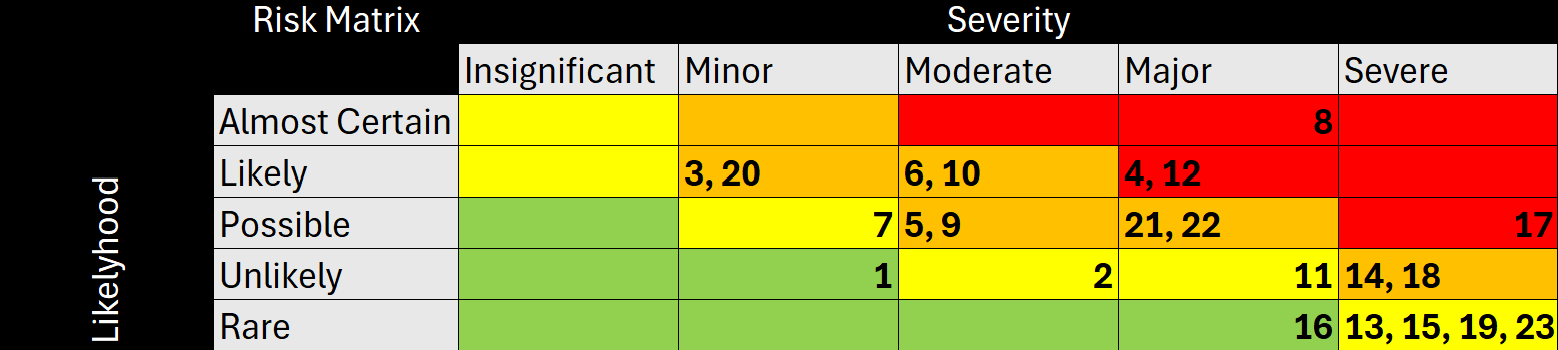
\includegraphics[width=0.95\textwidth]{./content/img/Mth/ProjectManagement/Risks_Mth_Initial.png}
    \caption{Initial risk assessment at the beginning of the Master Thesis.}
    \label{tab:mth_initial_risk_assessment}
\end{table}



\subsubsection*{Previous heat map}
As a reference for the continued risk management over the course of the entire initiative, the following heat map shows the status at the beginning of the second project. This illustrates that, over the course of the initiative, risks have been added and are now evaluated differently by the project team.

\begin{table}[H]
    \centering
    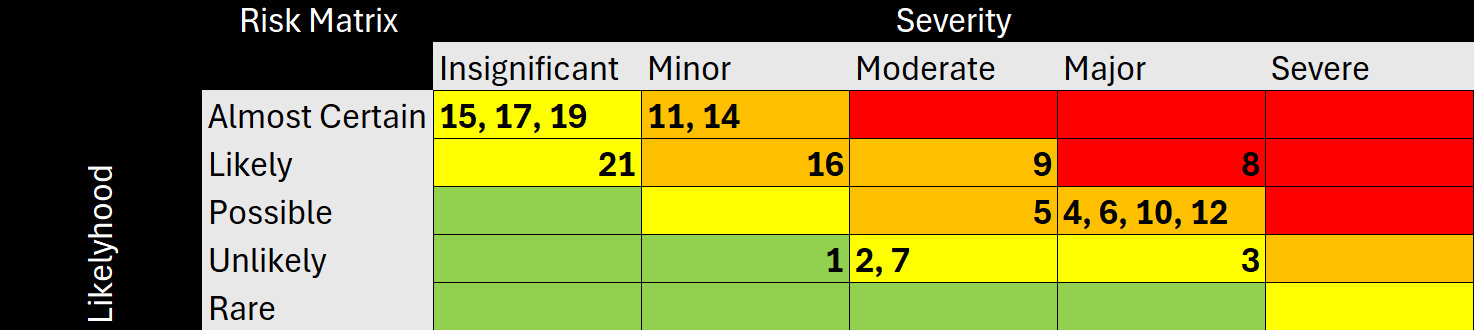
\includegraphics[width=0.95\textwidth]{./content/img/Mth/ProjectManagement/Risks_Mth_Project1.png}
    \caption{Risk matrix from Project 1.}
    \label{tab:risks_sev_likely}
\end{table}



\subsection*{Risk strategies and mitigation strategies}

Risk strategies are the high level approaches to dealing with the risks, and the risk mitigations are the concrete plans developed to manage identified risks. In the following table, an overview of the individual risks is provided, including their selected treatment and a brief justification. Naturally, it is neither practical nor feasible to completely eliminate every risk; therefore, based on likelihood and severity, as well as the team’s \gls{riskappetite}, each risk was assigned one of the following strategies:

\begin{itemize}
\item \textbf{Accept} – the risk and its potential impact are acknowledged, but no measures are taken
\item \textbf{Reduce} – the risk is mitigated by applying additional measures to lower its impact or probability
\item \textbf{Transfer} – the responsibility for handling the risk is assigned to another party
\item \textbf{Avoid} – the project is adapted in a way that prevents the risk from materialising
\end{itemize}

\begin{longtable}{@{} C{1.2cm} L{2.5cm} L{4.5cm} L{2.5cm} L{5cm} @{}}
\caption{Risk Strategy and Treatment Plan}\label{tab:risk_treatment}\\

\toprule
\textbf{No.} & \textbf{Risk} & \textbf{Risk Description} & \textbf{Treatment} & \textbf{Treatment Description} \\
\midrule
\endfirsthead

\toprule
\textbf{No.} & \textbf{Risk} & \textbf{Risk Description} & \textbf{Treatment} & \textbf{Treatment Description} \\
\midrule
\endhead

\midrule
\multicolumn{5}{r}{\small Continued on next page} \\
\endfoot

\bottomrule
\endlastfoot


1 & Goal & Unclear question & Reduce & Define SMART goals. \\
2 & Goal & Unclear goals & Reduce & Describe which goals are within the scope. \\
3 & Time and Organisation & Insufficient expertise & Accept & Learning is part of the process, but additional time needs to be planned. \\
4 & Time and Organisation & Underestimated time/effort & Reduce & Phases and milestones are set up as progress checks. \\
5 & Time and Organisation & Other study projects & Accept & Use minimal time for other projects/classes. \\
6 & Time and Organisation & Work projects & Reduce & Reduce the risk by starting early and defining blockers for study work. \\
7 & Time and Organisation & Procrastination & Reduce & Start early. \\
8 & Human Resources & Unavailability of main project staff, e.g. due to illness & Reduce & This happened before the start. Provide the contact details of the partner working at BFH and document the situation in case it happens again. \\
9 & Human Resources & Unavailability of advisor, e.g. due to illness or accident & Transfer & The advisor should define an emergency replacement. \\
10 & Tech and Infrastructure & Software version/library/dependency & Accept & Run the code multiple times and use test cases, e.g. unit tests. \\
11 & Tech and Infrastructure & Hardware is damaged & Reduce & Second laptop; code and documentation on GitHub, Miro, Teams, and Outlook. \\
12 & Data and Research & Data related & Accept & No preparation is planned. \\
13 & Data and Research & Not reproducible work & Reduce & Document major steps, upload versions of the document to GitHub, and use Kanban in Miro to document tasks. \\
14 & Ethical and Legal & Plagiarism or incorrect citation & Reduce & Use citations and a bibliography. \\
15 & Ethical and Legal & Copyright & Accept & Declare sources in the bibliography. For Swiss Post sources, use only public documents. \\
16 & Communication and Cooperation & Bad communication with stakeholders or advisor & Reduce & Weekly advisor meetings (Jour Fixe). \\
17 & Communication and Cooperation & Insufficient exchange with external partners & Reduce & Include stakeholders in the Scrum team. \\
18 & Force Majeure & Unforeseen family crisis & Accept & Document it in the Miro calendar if it happens. \\
19 & Force Majeure & General force majeure & Accept & Document it in the Miro calendar if it happens. \\
20 & Unknown Process & The required management process is unknown & Reduce & Projects 1 and 2 established many of the required steps. However, it is still likely that something new may arise. \\
21 & Communication and Cooperation & Required resources are not available when needed, or responsibilities are unclear & Reduce & Schedule calls early and search for external resources before starting work blocks. \\
22 & Organisational & Changes pushed by the organisation & Accept & Change is constant; discussions with teams are required. \\
23 & Data and Research & Insufficient scientific contribution & Reduce & Provide continuous feedback and hold weekly calls to identify missing contributions early. \\

\end{longtable}

\subsection*{Implementation of risk mitigation strategies}
Identifying the key risks is the first step in the overall risk management approach; this is followed by defining measures for each of the risks. In the following table, the implementation of these measures is documented. The measures have been implemented according to the strategies and descriptions outlined above. Table \ref{tab:risk_actions} provides an overview of the actions taken and when they were carried out.


\begin{longtable}{@{}C{1cm}L{3.5cm}L{9cm}C{2.5cm}@{}}
\caption{Risk Strategy and Action Overview}\label{tab:risk_actions}\\

\toprule
\textbf{No.} & \textbf{Risk} & \textbf{Strategy Decision / What} & \textbf{When} \\
\midrule
\endfirsthead

\multicolumn{4}{c}{\bfseries \tablename\ \thetable{} -- continued from previous page} \\
\toprule
\textbf{No.} & \textbf{Risk} & \textbf{Strategy Decision / What} & \textbf{When} \\
\midrule
\endhead

\midrule
\multicolumn{4}{r}{\small Continued on next page} \\
\bottomrule
\endfoot

\bottomrule
\endlastfoot


1 & Unclear question & Reduce: SMART goals have been defined in the research section. & 24.10.2026 \\
2 & Unclear goals & Reduce: The introduction describes which parts of the initial project description are included in this document. & 24.10.2026 \\
3 & Insufficient expertise & Accept: Nothing done. & 24.10.2026 \\
4 & Underestimated time/effort & Reduce: Phases and milestones are set up as progress checks. & 24.10.2026 \\
5 & Other study projects & Accept: Nothing done. & 24.10.2026 \\
6 & Work projects & Reduce: Discussed availability with the other team, added blockers to the work calendar, invited the work account to the Jour Fixe meeting series, set weekend blockers in the study account, and researched optimal or minimal study plans with ChatGPT. & 24.10.2026 \\
7 & Procrastination & Reduce: Work on the project started on 14.09.2026, with the first meeting with the expert in the same week. & 24.10.2026 \\
8 & Unavailability of main project staff, e.g. due to illness & Reduce: The partner's contact details were provided in Teams and added to the Miro board. & 24.10.2026 \\
9 & Unavailability of advisor, e.g. due to illness or accident & Transfer: Asked for a contact; Jürgen Vogel was confirmed as the replacement. & 24.10.2026 \\
10 & Software version/library/dependency & Accept: Nothing done. & 24.10.2026 \\
11 & Hardware is damaged & A second laptop is available at home. The LaTeX document is a GitHub project, and documentation is stored in Miro. The work laptop can also be used for most tasks but does not have LaTeX installed. & 24.10.2026 \\
12 & Data related & Accept: Nothing done. & 24.10.2026 \\
13 & Not reproducible work & Reduce: GitHub project for the LaTeX document. & 24.10.2026 \\
14 & Plagiarism or incorrect citation & Reduce: JabRef is used as a GUI for the bibliography, and Biber is used for compilation. & 24.10.2026 \\
15 & Copyright & Accept: Nothing done. & 24.10.2026 \\
16 & Bad communication with stakeholders or advisor & Reduce: Jour Fixe has been set up. & 24.10.2026 \\
17 & Insufficient exchange with external partners & Reduce: Maintain communication channels even when changing teams. & 24.10.2026 \\
18 & Unforeseen family crisis & Accept: Nothing done. & 24.10.2026 \\
19 & General force majeure & Accept: Nothing done. & 24.10.2026 \\
20 & The required management process is unknown & Reduce: It is still important to address new requirements as soon as they appear. & 24.10.2026 \\
21 & Required resources are not available when needed, or responsibilities are unclear & Reduce: Search for external resources before starting your own work. & 24.10.2026 \\
22 & Changes pushed by the organisation & Accept: Exchange information with teams. & 24.10.2026 \\
23 & Insufficient scientific contribution & Reduce: Addressed as part of the Jour Fixe. & 24.10.2026 \\

\end{longtable}

\subsection*{Ongoing risk monitoring}
A critical step in the risk management process is ongoing monitoring. Monitoring the risks ensures that the defined measures remain valid and that any risks that may materialise are identified. If a new risk is identified or causes a disruption to the project, it will be documented. Additionally, an appropriate measure to handle its impact will be defined. Monitoring of the risks will be performed every second Friday of each month. Detailed information about the risk monitoring process is provided in the appendix \ref{RiskMonitoring}.
These risk check-ins will contain the following information:

\begin{itemize}
\item Number of risk: same as in the tables above
\item Name of risk: same as in the tables above
\item Occurred: did the risk occur (yes or no)?
\item Details: what happened?
\item Cause: brief analysis of why it happened
\item Measures taken: what measures have been taken?
\item Measure date: on what date were measures taken?
\end{itemize}

\subsection*{Risk review at project completion}

Finally, a review of the risks will be held at the end of the project. This will address which risks came into effect and which did not. Additionally, changes to the perception of the risks will be documented at the start of the master thesis. 
